\documentclass{llncs}

\usepackage[utf8]{inputenc}
\usepackage{url}
\usepackage{graphicx}
\graphicspath{{./images/}}

\title{Using human-machine hybrid workflow in crowdsourcing open geospatial data}

\author{Gianfranco Cecconi}
\institute{University of Southampton \email{gc1a13@soton.ac.uk}}

\date{December 2015}

\begin{document}

\maketitle

[MAX 18 PAGES]

\section{Introduction}

\subsection{Crowdsourcing}

    Crowdsourcing is {[}...{]}. More generally {[}SOME LIGHTWEIGHT REFERENCE TO WHAT A SOCIAL MACHINE IS{]} [{[}BLAH BLAH SOCIAL MACHINES AS POSSIBLY ONE OF THE ONLY WAYS TO SOLVE PROBLEMS LIKE THIS + SOME EXCUSE TO CITE \cite{OReilly:2015uo}{]}

\subsection{Crowdsourcing Geographic Information}

    Among the many applications of crowdsourcing is the collection and maintenance of geospatial data, or "Geographic Information" (GI), as it is commonly referred to in literature.
    
    Although it is commonly recognised for GI to have a significant economic and social value \cite{Sui:2012uf}[THIS IS A REFERENCE TO AN ENTIRE BOOK, LIKELY UNSUITABLE], the effort national mapping and cadastre agencies (NMCAs) worldwide put into producing and updating cartography has been in decline for several decades \cite{ESTES:1994vz}. In the U.S., for example, the Geological Survey (USGS) no longer attempts to update its maps on a regular basis and the National Research Council promotes a vision in which {[}...{]} \cite{Committee:1993vp}.
    
    {[}Somewhere in the literature someone said that the emergence of VGI was actually suggested by one of those authorities{]}
    
    Crowdsourcing GI is then seen as the cost effective and "good enough" solution to this problem [CITATION OF SOME SCHOLAR SAYING THAT GOOD ENOUGH IS... GOOD ENOUGH]. The phenomenon of {\it Volunteered} Geographic Information (VGI) in particular was studied extensively since the term was coined \cite{Goodchild:2007vt}. Developing understanding of VGI was made possible by the success of services such as Wikimapia\footnote{\url{http://wikimapia.org/}.} or OpenStreetMap\footnote{\url{http://www.openstreetmap.org/}.}. The latter is likely the best known VGI-based mapping service available today.

\subsection{Open data}

    Open data is data that anyone can access, use and share\footnote{\url{http://theodi.org/faq}.}. 
    
    NMCAs, as governments and private organisations, are becoming more sensitive to the opportunities arising from publishing and re-using open data. In Great Britain, for example, since 2015 the local NMCA Ordnance Survey\footnote{\url{http://www.ordnancesurvey.co.uk/}.} has released in the open a substantial volume of data that was previously available to the public as commercial products only, e.g. "Open Names"\footnote{\url{https://www.ordnancesurvey.co.uk/business-and-government/products/os-open-names.html}.}, a place-name index, and "Open Roads"\footnote{\url{https://www.ordnancesurvey.co.uk/business-and-government/products/os-open-roads.html}.}, the generalised geometry and network connectivity of the road network.
    
    The availability of such high quality and authoritative sources becomes a substantial enabler for the creation of new GI. There were geospatial data could only be created from scratch - as in OpenStreetMap's case when it was started in the UK in 2007 - it is now possible to rather focus the effort of the crowd on complementing the GI that is already available.

\subsection{Crowdsourcing open data}

    This work took place in the context of a larger research programme aimed at assessing the feasibility of building original open data by using non-expert human contributions, technology systems and, where available, other pre-existing open data. 
    
    Although most of the effort of producing and releasing open data is commonly expected of governments and businesses, there are industry sectors and domains of knowledge where resistance to change can halt or substantially slow down this process. Demand and offer for open data is strongly suppressed, for example, due to failure in recognising open data-enabled business models, restrictive legislative and patent systems, or charging for public datasets \cite{shadboltpaf}. 
    
    The assumption at the base of our research is that the people's contribution is necessary to address this problem. People can be enabled, through technology, to capture and curate data, alongside what is already published by governments and businesses. Crowdsourcing is just one of the formulae by which socio-technical systems can be built for this purpose. This contribution is instrumental to delivering and curating the open data needed to build and operate a comprehensive {\it national information infrastructure} (NII).

\subsection{Challenges of crowdsourcing geospatial data}

    Two groups of challenges are relevant to the availability of good quality geospatial open data: on one side, exploiting it to improve the quality and enhance the functionality of pre-existing VGI initiatives, and, on the other, unleash completely new products and services.
    
    [SHOULD I WRITE MORE ABOUT THE OTHER CHALLENGES, TOO?]
    
    Completeness is a key element in the quality of geospatial data. In this paper we propose a method to improve the coverage of existing geospatial data where - for any reason - it is not possible to get volunteers to survey one specific geographical area or provide more detail than what is available already. This was described, for example, by **** , observing how OpenStreetMap volunteers naturally tend to avoid ***.
    
    {[}
    Add
    \begin{itemize}
    	\item {[}rationale of why we thought this was relevant, some justification in literature review{]}
    	\item {[}novelty of what we propose{]}
    \end{itemize}
    {]}
    
    {(}...{)}

\subsection{The Open Legal Address File}

    The main use case for this research is the attempt of creating a new geospatial dataset that is functionally equivalent to the "Postcode Address File" or "PAF"\footnote{PAF is a registered trademark by Royal Mail plc. For convenience we won't show the registered trademark sign "\textregistered" in this document every time we refer to it.}: a commercial dataset listing all known valid addresses and postcodes for the UK at a given point in time. 
    
    An act of law\footnote{The Postal Service Act 2000, part VII, article 116 \cite{postalserviceact2000}.} makes PAF ownership of the Royal Mail: the ex-postal service monopolist in the UK, now a public limited company with only a 30\% of shares controlled by the Government\footnote{The Postal Services Act 2011 plans to reduce the Government control down to 10\% \cite{postalserviceact2011}.}. The same act of law requires Royal Mail to make PAF available on "reasonable terms" to "any person who wishes to use it".
    
    To this day, though, the "reasonable terms" translated only into PAF being made available by Royal Mail and its resellers as a commercial product\footnote{As an end user who wants to access PAF's data one may incur Royal Mail licence fees going from \pounds0.012 per transaction on a public website to \pounds90,000 per year for unlimited internal use by a corporate group. Even charitable organisation may not take advantage of free PAF access unless their income is less than \pounds10m/year.}. This is considered an anomaly by many, as "reasonable terms for the external use of PAF data by third parties should be no more than the marginal cost of distribution (...)" \cite{odugresponse}. 

    To further limit the opportunities for PAF to be made open, in October 2013 Royal Mail and its assets were privatised, including PAF\footnote{\url{http://www.theguardian.com/uk-news/2014/mar/17/royal-mail-privatisation-ministers-rebuked-selling-data}}. The UK Parliament House of Commons' Public Administration Select Committee, just a few month later, called this "unacceptable and unnecessary" and recognised that PAF's "disposal for a short-term gain will impede economic innovation and growth" \cite{pascod}.

    This makes the opportunity of creating an alternative to PAF an ideal case study. We will call this the "Open Legal Address File", or "OLAF". The term "legal addresses" refers to all addresses that are, by law, in the public domain, hence have no restrictions in terms of intellectual property or privacy protection and can be published as open data\footnote{Legal addresses belong to either or both of the following two categories: a) they are the addresses of current or past UK residents who are or were registered on the public electoral register, and b) they are the addresses of past or present UK companies that are or were registered at the relevant British registrar, such as Companies House for England and Wales.}.

    {[}Definition of address{]}
    
    Many complementary and/or alternative strategies are possible and need to be used jointly to build OLAF. Among these is the opportunity to re-use published open datasets of addresses so to infer the existence of more addresses. 
    
    E.g. it is intuitive that if some source refers to the existence of house numbers 3, 5 and 9 in some street, and all are associated to the same postcode, it is very likely that number 7 exists as well and is associated to the same postcode\footnote{House numbering and postcode association are heavily dependant of the conventions used in the country the problem is applied to. This paper always refers to the UK conventions.}. It is shown experimentally that the method is effective, as it can produce large volumes of addresses from available open data\footnote{This was tested against the single largest known source of addresses open data for England and Wales: Land Registry's "Price Paid Data". See \url{https://www.gov.uk/government/collections/price-paid-data}.}.
    
    The experiments described in this paper implement the above strategy only, and  use crowdsourcing to validate sets of inferred addresses, as participants are asked to virtually survey the streets using pictures sourced from Google Street View.
    
    It has to be noted that not all existing house numbers are visible by surveying a street. E.g. there are no obligations in the UK to affix a house number or house name sign. Moreover, some of the house numbers may be associated to dwellings that are not visible unless the property is accessed, beyond what Google Street View's photos can capture.
    
    {(}...{)}

\section{Crowdsourcing addresses: our approach}

\subsection{The social machines mix}

    Although the OLAF data is conceptually simple, assembling such a large dataset while assuring sufficient quality is a complex task, even when starting from such valuable pre-existing open data such as Ordnance Survey's offering.
    
    It is our hypothesis that, to make the best use of pre-existing open data and potentially available technology and human resources, such a problem can be decomposed in a series of complementary sub-problems targeting parts of its scope, each addressed by a dedicated socio-technical system, or social machine. This decomposition can take place over several iterations, hence creating a hierarchy of systems. 

    \begin{figure*}
    	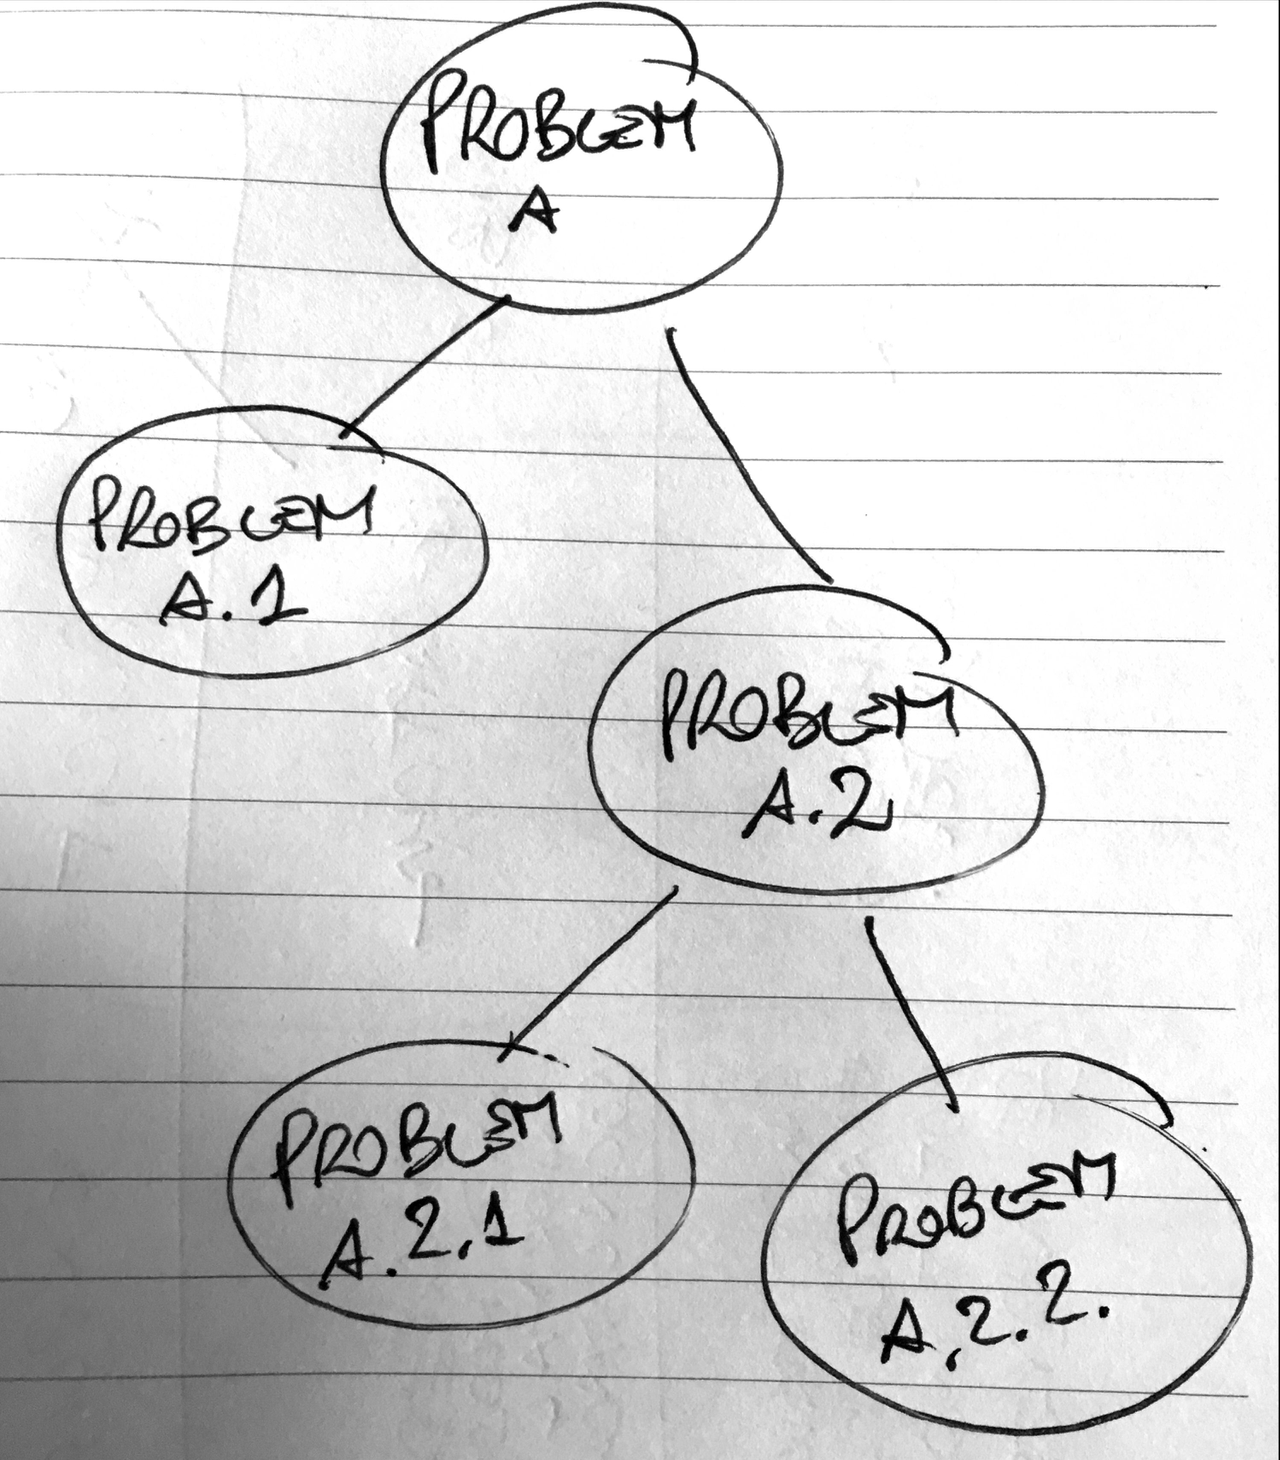
\includegraphics[width=0.95\textwidth]{social-machine-mix-1.png}
    	\caption{This picture should not be here, but apparently it is a nightmare in LaTeX.}
    	\label{fig:some_figure}
    \end{figure*}

    The open data available at the moment of writing from Ordnance Survey make it possible to divide the creation of OLAF in two


\subsection{Task model}

    The following is a description of the approach that was used for crowdsourcing addresses, that is common to all experimental conditions that were tested.
    
    \textbf{Requester.} The Requester desires to validate the existence of a series of house numbers (e.g. "3" or "7A") in a specified street. Those were previously inferred algorithmically from the observation of \textit{existing} house numbers, as sourced from published open datasets\footnote{See the GitHub repository at \url{https://github.com/Digital-Contraptions-Imaginarium/OLAF-yr2_reference_data} to learn about the reference open data we used, and the repository at \url{https://github.com/Digital-Contraptions-Imaginarium/OLAF-yr2_inference_data} for the inference algorithms.}. When the pictures in the survey tool are of insufficient quality to be read intelligibly (e.g. a house number could be "7A" but it is not clear) it is useful to the Requester to be informed of that. The Requester requires the help of human agents to carry out the tasks, that we will call Workers in the following.
    
    \textbf{Task.} Each HIT (Human Intelligence Task) consists of verifying the existence in a given street of a given specific tuple of inferred house numbers {[}SOME MATHS SYMBOLS HERE{]} that is a subset of the whole set of inferred house numbers for that street {[}SOME MATHS SYMBOLS HERE{]}. 
    
    \textbf{Strategy.} 
    {[}TO BE WRITTEN, DEPENDS ON THE EXPERIMENT SCENARIOS DEFINITION.{]}
    
    \textbf{Crowd $\rightarrow$ Worker.} Each Worker performs her task by declaring, for each house number in the given tuple and street, if a) it can be found by using the survey tool, b) it can't be found or c) it cannot be said with certainty (e.g. if some of the pictures are blurred and could correspond to the house number being searched). Multiple Workers are asked to validate the same tuple and the resulting data is chosen through majority voting.
    
    \textbf{Reliability.} When collecting data to build a dataset that is intended to be published under an open licence, the option to assess its \textit{quality} by comparison with other sources is often not available, for many reason. An alternative source of the same data could simply not be available. Moreover, from an intellectual property perspective, the comparison could make the former "derivative work" of the latter, hence compromising the purpose{[}SOME REFERENCE OR FOOTNOTE TO PUT MORE MEAT AROUND THIS POINT{]}. 
    
    What is possible, instead, is to estimate the \textit{reliability} of the crowdsourced data, independently of any actual knowledge of other sources and/or the ground truth. 
    
    In OLAF's case, the approach described is considered equivalent to what is used for crowdsourcing the acquisition of labels for data items when the labelling is imperfect, that is extensively covered in literature, e.g. in \cite{sheng2008get} or \cite{Welinder:2010vkb}{[STILL HAVE TO READ THE LATTER{]}. 
    
    The quality of the Workers' contribution could be measured by using gold standard tasks \cite{Oleson:2011tx}, e.g. asking them to validate sets of house numbers whose existence is already known. Because of the elementary complexity of the tasks, though, it was assumed that anything standing between the Worker and the actual required tasks would hinder their contribution in volume and quality and compromise furtherance.
    
    Lacking an assessment of the individual Worker's reliability, the option of preferring the best individual Workers vs using multiple labellers becomes unavailable, hence the need to use majority voting. 
    
    For simplicity, all Workers are considered equivalent from a reliability perspective, and the quality of their individual output assumed $ > 0.5 $, so that the \textit{uniform labeller quality} (see \cite{sheng2008get}) of the data chosen through majority voting increases as the number of labellers is increased.

\subsection{Recruitment}
\subsection{Design}
\subsection{The virtual survey tool}

    Some text before.
    
    \begin{figure*}
    	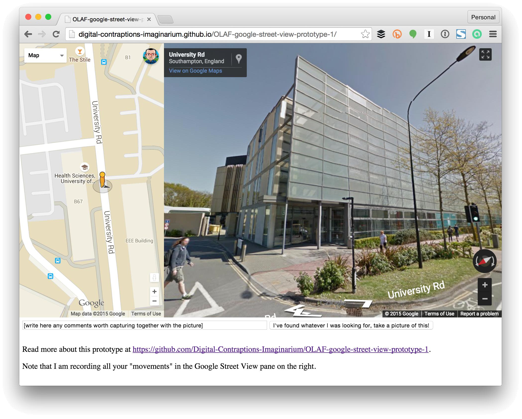
\includegraphics[width=0.95\textwidth]{some_picture.png}
    	\caption{This picture should not be here, but apparently it is a nightmare in LaTeX.}
    	\label{fig:some_figure}
    \end{figure*}
    
    \paragraph{}
    
    Some text after.
	
\subsection{Scalability}

    [THE CALL FOR PAPER EXPLICITLY SAYS THAT "EVIDENCE OF USE IN PRACTICE AND/OR DEMONSTRATION OF SCALABILITY IS REGARDED AS A PLUS"]

\subsection{{[}description of additional conditions to test X{]}}
\subsection{{[}description of additional conditions to test Y{]}}

\section{Experiment design}

\subsection{Research hypothesis}
\subsection{Dataset}
\subsection{Evaluation metrics}
\subsection{Experimental conditions}

\section{Results}

\section{Literature review}

\section{Discussion and conclusion}

\section*{Acknowledgments}

{[}The standard EPSRC acknowledgement formula + something about the external reviewers?{]}

\documentclass{article}
\usepackage{url}
\begin{document}
\nocite{*}
\bibliography{main}
\bibliographystyle{splncs03}
\end{document}


\end{document}

